\documentclass{beamer}
\usepackage{graphicx}

\usetheme{Ilmenau}

\usepackage{float}
\usepackage{tikz}
\usepackage{amsfonts}
\usepackage{amsmath}
\usepackage{bibentry}
\usepackage{setspace}
\usepackage{amssymb}
\usepackage{mathtools}
\usepackage{xcolor}
\usepackage{mathrsfs}
\usepackage{soul}
\usepackage{algorithm}
\usepackage{algpseudocode}
\usepackage{spverbatim}
\usepackage{multicol}
\usepackage{fancyvrb}
\usepackage[super]{nth}
\usepackage{listings}
\usepackage{linegoal}
\usepackage{calc}
\usepackage{tikz-qtree}
\usepackage{forest}
\graphicspath{ {figures/} }

\usetikzlibrary{positioning,calc,arrows.meta}%arrows is deprecated

\newtheorem{plain}{Remark}

\addtobeamertemplate{navigation symbols}{}{%
    \usebeamerfont{footline}%
    \usebeamercolor[fg]{footline}%
    \hspace{1em}%
    \insertframenumber/\inserttotalframenumber
}

\setbeamercolor{footline}{fg=blue}
\setbeamerfont{footline}{series=\bfseries}

\title{Statically Scheduling Circular Remote Attribute Grammars}
\newcommand{\enquote}[1]{``#1''}

\newcommand{\emptyline}{\vspace{0.3cm}}
% A subtitle is optional and this may be deleted
% \subtitle{Lattice based key-exchange}

\author[Seyedamirhossein Hesamian]{Seyedamirhossein Hesamian \texorpdfstring{\\{\small Advisor: Dr. Boyland}}{}}



\institute[UW-Milwaukee] % (optional, but mostly needed)
{
  Department of Computer Science\\
  University of Wisconsin Milwaukee
}
% - Use the \inst command only if there are several affiliations.
% - Keep it simple, no one is interested in your street address.

\date{Winter 2021}

\newcommand{\newlinevspace}{\vspace{\baselineskip}}



% - Either use conference name or its abbreviation.
% - Not really informative to the audience, more for people (including
%   yourself) who are reading the slides online

\subject{Theoretical Computer Science}
% This is only inserted into the PDF information catalog. Can be left
% out. 

% If you have a file called "university-logo-filename.xxx", where xxx
% is a graphic format that can be processed by latex or pdflatex,
% resp., then you can add a logo as follows:

\pgfdeclareimage[height=0.5cm]{university-logo}{university-logo-uwm}
\logo{\pgfuseimage{university-logo}}

\algdef{SE}[DOWHILE]{Do}{DoWhile}{\algorithmicdo}[1]{\algorithmicwhile\ #1}%

\newcommand{\AlgMultiline}[1]{
\parbox[t]{\dimexpr\linewidth-\csname ALG@tlm\endcsname+\algorithmicindent}{\raggedright\hangindent\algorithmicindent%
            #1 }}
            
\setbeamertemplate{mini frames}{}

% Let's get started
\begin{document}

\begin{frame}
  \titlepage
\end{frame}

\begin{frame}{Outline}
\tiny
  \tableofcontents
  % You might wish to add the option [pausesections]
\end{frame}



\section{Introduction}

\begin{frame}{Importance of Attribute Grammars}{Applications mainly in compiler construction}
Primary application:

\begin{itemize}
    \item Program Analysis
        \begin{itemize}
            \item  Type Checking
            \item Control-Flow Analysis
        \end{itemize}
    \item Solving problems over AST
        \begin{itemize}
            \item  Nullable, First and Follow
        \end{itemize}
\end{itemize}

\emptyline

Other applications:
\begin{itemize}
    \item Natural Language Processing \cite{10.1007/978-3-642-25324-9_25}
    \item Model-driven engineering \cite{schone2020connecting}
    \item Testing Services \cite{habibisharif}
\end{itemize}
\end{frame}


\begin{frame}{Motivation}{Simplest form of attribute grammar}
Math expression consisting of addition \& multiplication

\[ 1 \times 2 + 3  \]

\newlinevspace

How to represent this as a \alert{CFG} with correct order of operation?
\end{frame}


\begin{frame}[fragile=singleslide]{Motivation}{Binary Expression CFG}

How to represent the \alert{final value} as an attribute grammar?

\begin{multicols}{2}
\begin{Verbatim}[fontsize=\small]
E -> E + T
  val = ?

E -> T
  val = ?




T -> T * F
  val = ?

T -> F
  val = ?

F -> digit
  val = ?
\end{Verbatim}
\end{multicols}
\end{frame}


\begin{frame}[fragile=singleslide]{Motivation}{Pure-S AG}

This is an example of \alert{purely synthesized} attribute grammar

\begin{multicols}{2}
\begin{Verbatim}[fontsize=\small]
E -> E + T
  E0.val = E1.val + T.val

E -> T
  E.val = T.val




T -> T * F
  T0.val = T1.val * F.val

T -> F
  T.val = F.val

F -> digit
  F.val = digit.lexical_val
\end{Verbatim}
\end{multicols}

\end{frame}




\begin{frame}{Motivation}{Derivation tree}
Arrows represent \alert{direction} of flow of attribute values:

$\to$ \alert{bottom-up} propagation

\begin{center}
\scalebox{0.75}{\begin{forest}
  [
    E, name=11
    [E,name=7 [T, name=6 [T,name=3 [F,name=2 [digit, name=1]]  ][*][F, name=5 [digit, name=4]  ]]]
    [+]
    [T, name=10 [F, name=9  [digit, name=8 ]]]
  ]
  \draw[->,dashed] (1) to[out=north west,in=south west] (2);
  \draw[->,dashed] (2) to[out=north west,in=south west] (3);
  \draw[->,dashed] (3) to[out=north west,in=west] (6);
  \draw[->,dashed] (4) to[out=north east,in=south east] (5);
  \draw[->,dashed] (5) to[out=north east,in=east] (6);
  \draw[->,dashed] (6) to[out=north west,in=south west] (7);
  \draw[->,dashed] (8) to[out=north east,in=south east] (9);
  \draw[->,dashed] (9) to[out=north east,in=south east] (10);
  \draw[->,dashed] (7) to[out=north west,in=west] (11);
  \draw[->,dashed] (10) to[out=north east,in=east] (11);
\end{forest}}    
\end{center}

\end{frame}





\begin{frame}{Attribute Grammars}{Extensions to original Knuth paper}

\begin{itemize}
    \item \alert{Classical Attribute Grammar} Introduced by Knuth in \cite{Knuth68semanticsof}
    \item \alert{Ordered} Attribute Grammar Introduced by Kastens in \cite{10.1007/BF00288644}
    \item \alert{Circular} Attribute Grammar Introduced by Farrow in \cite{10.1145/13310.13320}
    \item \alert{Remote} Attribute Grammar Introduced separately by Boyland in \cite{10.5555/924544, Boyland05remoteattribute} and Hedin \cite{DBLP:journals/informaticaSI/Hedin00}
    \item \alert{Circular Remote} Attribute Grammar Introduced by Hedin in \cite{10.1016/j.scico.2005.06.005}
\end{itemize}
	
\end{frame}


\begin{frame}{Goal}{End-goal of this thesis}
    
\begin{itemize}
    \item \alert{Statically scheduling} circular remote attribute grammars
    \begin{itemize}
        \item Modifying \alert{APS attribute grammar system} to handle this extension
        \item Testing it against circularly defined problems like First and Follow and \alert{Cool semantic analyzer}
    \end{itemize}
\end{itemize}
    
\end{frame}

\begin{frame}{Impact}{Advancing knowledge}
    
\begin{itemize}
    \item This has NOT been done before
    \begin{itemize}
        \item Not even static evaluator for \alert{circular AG}
    \end{itemize}
    \item Completes the attribute grammars for practical use
\end{itemize}    

\end{frame}
\section{Related Works}

\begin{frame}{JastAdd}{Closely related attribute grammar system}
Introduced by Hedin in \cite{DBLP:journals/entcs/HedinM01}
		
\begin{itemize}
    \item \alert{Imperative}
    \item Demand Evaluation
    \item Supports collections
    \item Supports Remote Attribute Grammars
    \item \alert{Supports Circular Remote Attribute Grammar} via an artifact
    \item Syntactically close to Java
\end{itemize}

\end{frame}

\begin{frame}{APS}{Main focus of this thesis}
Introduced by Boyland in \cite{10.5555/924544}
		
\begin{itemize}
    \item \alert{Declarative}
    \item \alert{Static Evaluation}
    \item Demand Evaluation
    \item Supports collections
    \item Supports Remote Attribute Grammars
    \item Target code generation to Scala and C++
\end{itemize}

\end{frame}

\begin{frame}{Other Declarative Program Analysis Tools}{Not necessary related to attribute grammars}

\begin{columns}
\column{.5\textwidth}
\alert{Datalog}
\begin{itemize}
    \item Logic programming
    \item Weakly typed
    \item Syntactically subset of Prolog
    \item Not lattice support
\end{itemize}
\column{.5\textwidth}
\alert{FLIX}
\begin{itemize}
    \item ML-family
    \item Strongly typed
    \item Lattice support
\end{itemize}
\end{columns}

\end{frame}

\section{Definitions}

\subsection*{Preliminaries}

\begin{frame}{Context-Free Grammar (CFG)}{Foundation that attribute grammars built upon}

A grammar consists of:
\begin{itemize}
    \item a set of non-terminals, one of which is designated as the start variable
    \item a set of terminals
    \item a set of productions
\end{itemize}
\end{frame}

\begin{frame}[fragile=singleslide]{Example}{Grammar for a simple language}

\begin{multicols}{2}
\begin{Verbatim}[fontsize=\scriptsize]
program -> block

block -> "begin" decls stmts "end"

decls ->

decls -> decls decl

decl -> id ":" type ";"

type -> "Integer"

type -> "String"

stmts -> 

stmts -> stmts stmt

stmt -> block ";"

stmt -> expr := expr

expr -> INT_CONSTANT

expr -> STRING_CONSTANT

expr -> id
\end{Verbatim}
\end{multicols}


Source: \cite{Boyland1998AnalyzingDN}

\end{frame}



\begin{frame}[fragile=singleslide]{Example}{Derivation of this simple language}

\begin{Verbatim}[fontsize=\scriptsize,numbers=left,xleftmargin=5mm]
begin
   x : String;
   y : Integer;
	
   x := z;
   y := "hello world!";
end
\end{Verbatim}

\newlinevspace

\begin{itemize}
    \item Use of undeclared variable
    \item Type mismatch?
    \item Unused variable
\end{itemize}

\newlinevspace

$\to$ How to detect these issues using attribute grammars?
\end{frame}


\begin{frame}{Classical Attribute Grammar}{CFG + Rules}


A classical attribute grammar is a \alert{grammar} with the following added features:

\begin{itemize}
    \item Each symbol $X$ has a set of attributes $A(X)$
    \item $A(X)$ has two disjoint subsets
    \begin{itemize}
        \item $S(X)$, synthesized attributes, which are passed up the tree
        \item $I(X)$, inherited attributes which are passed down the tree
    \end{itemize}
    \item Set of local attributes associated with each production
    \item Each production of the grammar has a set of semantic functions
\end{itemize}

\end{frame}

\begin{frame}[fragile=singleslide]{Example}{Classical attribute grammar to find semantic errors in a program}


\begin{multicols}{2}
\begin{Verbatim}[fontsize=\fontsize{1}{1}\selectfont]
program -> block
	block.env = empty_env()
	program.msgs = block.msgs
	
block -> "begin" decls stmts "end"
	decls.envin = block.env
	stmts.env = decls.envout
	decls.uin = stmts.used
	block.used = decls.uout
	block.msgs = decls.msgs ++ stmts.msgs
	
decls ->
	decls.envout = decls.envin
	decls.uout = decls.uin
	decls.msgs = { }

decls -> decls decl
  decls1.envin = decls0.envin
  decl.envin = decls1.envout
  decls0.envout = decl.envout
  decl.uin = decls0.uin
  decls1.uin = decl.uout
  decls0.uout = decls1.uout
  decls0.msgs = decls1.msgs ++ decl.msgs

decl -> id ":" type ";"
  decl.envout = add_env(<id, type.shape>, decl.envin)
  decl.uout = decl.uin - id
  decl.msgs = if id in decl.uin then
                { }
              else
                { "unused: " + id }

type -> "Integer"
  type.shape = INT_SHAPE

type -> "String"
  type.shape = STR_SHAPE

stmt ->
  stmts.used = { }
  stmts.msgs = { }

stmts -> stmts stmt
  stmts1.env = stmts0.env
  stmt.env = stmts0.env
  stmts0.used = stmts1.used ++ stmt.used
  stmts0.msgs = stmts1.msgs ++ stmt.msgs

stmt -> block ";"
  block.env = stmt.env
  stmt.used = block.used
  stmt.msgs = block.msgs

stmts -> expr ":=" expr ";"
  expr1.env = stmt.env
  expr2.env = stmt.env
  stmt.used = expr1.used ++ expr2.used
  stmt.msgs = (if expr1.shape != expr2.shape then
                { "type mismatch" }
              else
                { }) ++ expr.msgs

expr -> INT_CONSTANT
  expr.shape = INT_SHAPE
  expr.used = { }
  expr.msgs = { }

expr -> STR_CONSTANT
  expr.shape = STR_SHAPE
  expr.used = { }
  expr.msgs = { }

expr -> id
  local shape = lookup(id, expr.env)
  expr.shape = shape
  expr.used = { id }
  expr.msgs = if shape == NOT_FOUND then
                { id + " not declared" }
              else
                { }
\end{Verbatim}
\end{multicols}

\end{frame}


\begin{frame}{Instantiated Attribute Grammar}{Attribute Grammar + Derivation}
Given a \alert{derivation} of grammar, an attribute grammar becomes \alert{instantiated}:
\begin{itemize}
    \item Set of instantiated semantic rules where each attribute \alert{occurrence} is replaced with attribute \alert{instance}
\end{itemize}

\end{frame}


\subsection*{Evaluations}

\begin{frame}{Evaluation}{Core concept}

Evaluation is a process of finding the \alert{values} of \alert{attribute instances}.

\end{frame}

\begin{frame}{Demand Evaluation}{Straightforward evaluation method}
\begin{definition}
Demand evaluation is a kind of evaluation where each attribute instance access requires a call to evaluate the corresponding instantiated semantic rule that defines it.
\end{definition}

\end{frame}


\begin{frame}[fragile=singleslide]{Example}{Simple yet abstract example of classical attribute grammar}
    
\begin{multicols}{3}
\begin{verbatim}
S -> A
  A.i1  = S.in
  A.i2  = A.s1
  S.out = A.s2




A -> A A
  A1.i1 = A0.i1
  A1.i2 = A1.s1
  A0.s1 = A1.s2
  A2.i1 = A0.i2
  A2.i2 = A2.s1
  A0.s2 = A2.s2

A -> epsilon
  A.s1 = A.i1 + 1
  A.s2 = A.i2 + 2
    
    
    
    
\end{verbatim}
\end{multicols}

Source: \cite{10.1145/225540.225544}
    
\end{frame}


\begin{frame}[fragile=singleslide]{Example}{Instantiated attribute grammar}

\[
\lefteqn{\underbrace{\phantom{S \rightarrow A}}_{n_0}} S \rightarrow
\lefteqn{\overbrace{\phantom{A \rightarrow A A}}^{n_1}} A \rightarrow 
\lefteqn{\underbrace{\phantom{A A \rightarrow \epsilon}}_{n_2}} A A \rightarrow \epsilon
\lefteqn{\overbrace{A \rightarrow \epsilon}^{n_3}}
\]


\begin{multicols}{3}
\begin{Verbatim}[fontsize=\scriptsize]
n0: S -> A
  r0 : n1.i1  = n0.in
  r1 : n1.i2  = n1.s1
  r2 : n0.out = n1.s2




n1: A -> A A
  r3 : n2.i1 = n1.i1
  r4 : n2.i2 = n2.s1
  r5 : n1.s1 = n2.s2
  r6 : n3.i1 = n1.i2
  r7 : n3.i2 = n3.s1
  r8 : n1.s2 = n3.s2

n2: A -> epsilon
  r9 : n2.s1 = n2.i1 + 1
  r10: n2.s2 = n2.i2 + 2
    
n3: A -> epsilon
  r11: n3.s1 = n3.i1 + 1
  r12: n3.s2 = n3.i2 + 2
\end{Verbatim}
\end{multicols}

The sequence of steps needed to evaluate $\alert{n_0.\mathit{out}}$:
$\alert{n_0.\mathit{out}} \to \alert{r_2}{:} n_o.\mathit{out} = n_1.s_2 \to \alert{r_8}{:} n_1.s_2 = n_3.s_2 \to \alert{r_{12}}{:}n_3.s_2 = \dots$

\end{frame}


\begin{frame}{Demand Evaluation}{Pros and cons}
Pros:
\begin{itemize}
    \item Can benefit form \alert{caching to prevent re-evaluation}
    \item Easy to implement
\end{itemize}

Cons:
\begin{itemize}
    \item Does not detect cycles before evaluation begins or \alert{may not terminate}
    \item Space complexity if \alert{caching} is used: $\mathcal{O}(|\hat{V}|)$
    \item Time complexity of: $\mathcal{O}(| \hat{V} | \times | \hat{R} |)$ (for classical AG)
\end{itemize}
\end{frame}


\begin{frame}{Schedule Evaluation}{Finding the order of evaluation of instantiated rules before evaluation runtime}

Given this \emph{schedule}, evaluate the AG:

\begin{equation}
\begin{split}
\mathit{schedule} = \Big \{\hat{r}_0 < \hat{r}_3 < \hat{r}_9 < \hat{r}_4 < \hat{r}_{10} < \hat{r}_5 < \hat{r}_1 < \hat{r}_6 \\
< \hat{r}_{11} < \hat{r}_7 < \hat{r}_{12} < \hat{r}_8 < \hat{r}_2 \Big \}    
\end{split}
\end{equation}

\begin{alertblock}{Observation}
Finding the schedule requires topological sort of attribute instances: $\mathcal{O}(| V +  E|)$ where $V = \hat{V}$ and $E = |\hat{V}  \times  \hat{R}|$
\end{alertblock}
\end{frame}


\begin{frame}{Schedule Evaluation}{Pros and cons}
Pros:
\begin{itemize}
    \item If scheduler finds a schedule, then evaluation \alert{will terminate}
    \item Easy to implement
    \item \alert{No re-evaluation}
    \item Better space complexity as caching is not used
    \item Time complexity of: $\mathcal{O}(| \hat{R} |)$ (for classical AG)
\end{itemize}

Cons:
\begin{itemize}
    \item Schedule \alert{works only for one derivation} of attribute grammar
\end{itemize}
\end{frame}


\begin{frame}{Schedule}{Total order of instantiated rules}
What makes a schedule (total order on instantiated rules) valid?

\newlinevspace

$\to$ \alert{No use of attribute instance before it is defined first}

\end{frame}



\begin{frame}{Static Evaluation}{Alternative evaluation method: Constructed independent of a derivation}

\begin{itemize}
    \item What if there was a way to \alert{statically} evaluate attribute grammars?
    \begin{itemize}
        \item Generate evaluator \alert{once} and would \alert{work for all possible derivations} of an attribute grammar.
    \end{itemize}
    \item What \alert{constraints} need to be true for such an attribute grammar to have a static evaluator?
    \item Does evaluation \alert{terminate}?
    \item How to verify if static evaluation is \alert{valid}?
\end{itemize}
\end{frame}



\begin{frame}{Visit Sequence Evaluation}{Static evaluator}

$\to$ \alert{Visit sequence evaluation} is a \alert{type of static evaluation}.

\newlinevspace

Pros:
\begin{itemize}
    \item Evaluation \alert{will terminate}
    \item Easy to implement
    \item \alert{No re-evaluation}
    \item Better space complexity as caching is not used
    \item Time complexity of: $\mathcal{O}(| \hat{R} |)$ (for classical AG)
    \item \alert{Practical}: can be generated independent of derivation
\end{itemize}

Cons:
\begin{itemize}
    \item Only works on \alert{$l$-ordered} class of attribute grammars
\end{itemize}
\end{frame}



\begin{frame}[fragile=singleslide]{Example}{Visit sequence evaluator}

$\to$ Set of \alert{recursive functions} where each function takes an \alert{instance of non-terminal} (derivation tree node)

\begin{multicols}{2}
\begin{Verbatim}[fontsize=\scriptsize]
visit_S(n: S -> A)
    A.i1 = S.in
    - visit_A_part1(A)
    A.i2 = A.s1
    - visit_A_part2(A)
    S.out = A.s2

visit_A_part1(n: A -> A A)
    A1.i1 = A0.i1
    - visit_A_part1(A1)
    A1.i2 = A1.s1
    - visit_A_part2(A1)
    A0.s1 = A1.s2
visit_A_part2(n: A -> A A)
    A2.i1 = A0.i2
    - visit_A_part1(A2)
    A2.i2 = A2.s1
    - visit_A_part2(A2)
    A0.s2 = A2.s2

visit_A_part1(n: A -> epsilon)
    A.s1 = A.i1 + 1

visit_A_part2(n: A -> epsilon)
    A.s2 = A.i2 + 1
    
\end{Verbatim}
\end{multicols}
\end{frame}


\begin{frame}{$l$-ORD}{$T(X)$: Total order of attributes for non-terminal $X$ }

\[  T(S) = \{ S.\mathit{in} < S.\mathit{out}  \}  \]

\[  T(A) = \{ A.i_1 < A.i_2 < A.s_1 < A.s_2 \}  \]

\newlinevspace

$\to$ AG is $l$-ordered if exists a $T(X)$  for all non-terminal $X \in N$ such that its \alert{compatible} with $\mathit{Ord}(\mathit{AO}(p))$ and $\mathit{Ord}(R(p))$ where $p: X \rightarrow \alpha$. 

\end{frame}

% \begin{frame}{$l$-ORD}{Definition}


% \end{frame}

\begin{frame}{Visit Sequence}{Protocol}

\begin{definition}
A \emph{Protocol} $\Pi(X)$ is an \alert{ordered partition of attributes} for each non-terminal $X \in N$, where it can include an empty set or multiple synthesized or inherited attributes.
\end{definition}

\newlinevspace

\begin{examples}
For example, $\Pi(A)$ is the following:
\[ \Pi(A) = \Big\{ \{ A.i_1, A.s_1 \} < \{ A.i_2, A.s_2 \} \Big\} \]
\end{examples}

Visit Sequence has to be compatible with $\mathit{Ord}(R(p))$ and $\Pi(X_i)$

\end{frame}


% \begin{frame}{Visit Sequence Evaluation}{Visit sequence $\mathscr{V}(p)$}


% \end{frame}


% \begin{frame}{Visit Sequence Evaluator}{Interpreter style program that used visit sequence}

% \end{frame}




\begin{frame}{Visualization Tools}{Dependency graph}

\begin{figure}[htbp]
    \centering
    \resizebox{.8\textwidth}{!}{
    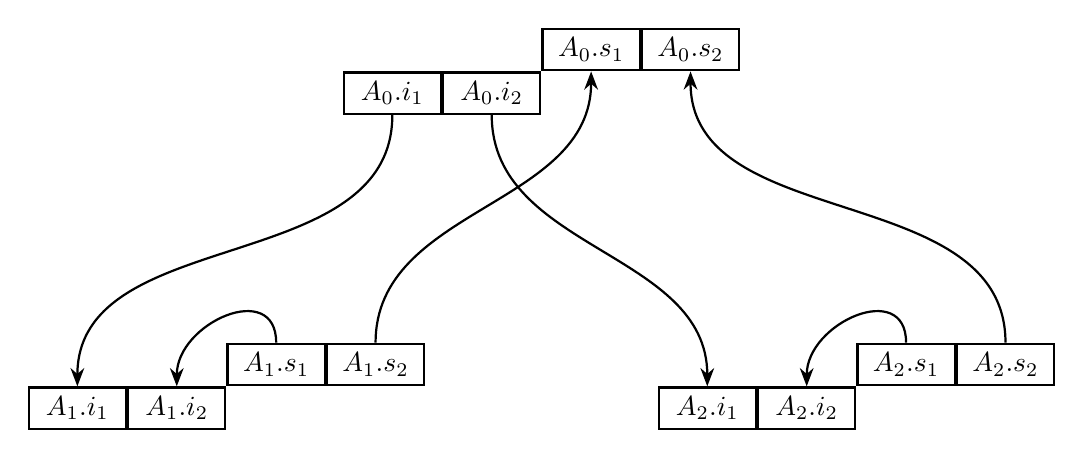
\begin{tikzpicture}[->,>=Stealth,auto,
        thick,main node/.style={draw, rectangle, align=center, text width=1cm}]

\node[main node, ] (1) at (-2,4)   {$A_0.i_1$};
\node[main node, anchor=north west] (2) at(1.north east) {$A_0.i_2$};
\node[main node, anchor=south west] (3) at(2.north east) {$A_0.s_1$};
\node[main node, anchor=north west] (4) at(3.north east) {$A_0.s_2$};


\node[main node, ] (5) at (-6,0)   {$A_1.i_1$};
\node[main node, anchor=north west] (6) at(5.north east) {$A_1.i_2$};
\node[main node, anchor=south west] (7) at(6.north east) {$A_1.s_1$};
\node[main node, anchor=north west] (8) at(7.north east) {$A_1.s_2$};

\node[main node, ] (9) at (2,0)   {$A_2.i_1$};
\node[main node, anchor=north west] (10) at(9.north east) {$A_2.i_2$};
\node[main node, anchor=south west] (11) at(10.north east) {$A_2.s_1$};
\node[main node, anchor=north west] (12) at(11.north east) {$A_2.s_2$};

\draw (12.north) to[out=90, in=-90, looseness=1] (4.south);
\draw (2.south) to[out=-90, in=90, looseness=1] (9.north);
\draw (8.north) to[out=90, in=-90, looseness=1] (3.south);
\draw (1.south) to[out=-90, in=90, looseness=1] (5.north);

\draw (11.north) to[out=90, in=90, looseness=1.5] (10.north);
\draw (7.north) to[out=90, in=90, looseness=1.5] (6.north);


\end{tikzpicture}}

    \caption{Dependency graph $\mathit{DG}_{p: A \rightarrow A A}$}
\end{figure}

\end{frame}

\begin{frame}{Visualization Tools}{Augmented dependency graph}

\begin{figure}[htbp]
    \centering

    \resizebox{.8\textwidth}{!}{
    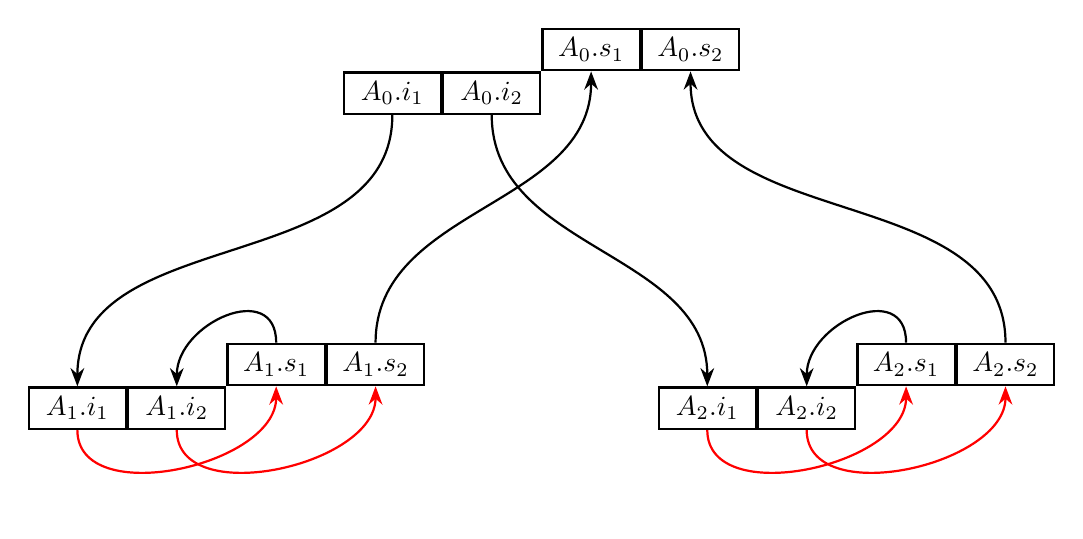
\begin{tikzpicture}[->,>=Stealth,auto,
        thick,main node/.style={draw, rectangle, align=center, text width=1cm}]

\node[main node, ] (1) at (-2,4)   {$A_0.i_1$};
\node[main node, anchor=north west] (2) at(1.north east) {$A_0.i_2$};
\node[main node, anchor=south west] (3) at(2.north east) {$A_0.s_1$};
\node[main node, anchor=north west] (4) at(3.north east) {$A_0.s_2$};


\node[main node, ] (5) at (-6,0)   {$A_1.i_1$};
\node[main node, anchor=north west] (6) at(5.north east) {$A_1.i_2$};
\node[main node, anchor=south west] (7) at(6.north east) {$A_1.s_1$};
\node[main node, anchor=north west] (8) at(7.north east) {$A_1.s_2$};

\node[main node, ] (9) at (2,0)   {$A_2.i_1$};
\node[main node, anchor=north west] (10) at(9.north east) {$A_2.i_2$};
\node[main node, anchor=south west] (11) at(10.north east) {$A_2.s_1$};
\node[main node, anchor=north west] (12) at(11.north east) {$A_2.s_2$};

\draw (12.north) to[out=90, in=-90, looseness=1] (4.south);
\draw (2.south) to[out=-90, in=90, looseness=1] (9.north);
\draw (8.north) to[out=90, in=-90, looseness=1] (3.south);
\draw (1.south) to[out=-90, in=90, looseness=1] (5.north);

\draw (11.north) to[out=90, in=90, looseness=1.5] (10.north);
\draw (7.north) to[out=90, in=90, looseness=1.5] (6.north);

\draw[red] (5.south) to[out=-90, in=-90, looseness=1] (7.south);
\draw[red] (6.south) to[out=-90, in=-90, looseness=1] (8.south);
\draw[red] (9.south) to[out=-90, in=-90, looseness=1] (11.south);
\draw[red] (10.south) to[out=-90, in=-90, looseness=1] (12.south);

\end{tikzpicture} }

    \caption{\small Augmented dependency graph $\mathit{DG}_{p: A \rightarrow A A}$ with SNC summary edges}
\end{figure}

\end{frame}


\begin{frame}{Ordered AG Test}{Test if visit sequence evaluator exists (efficiently)}
By definition, there exist a visit sequence for \alert{$l$-ordered} attribute grammars but membership test is \alert{NP-complete} \cite{ENGELFRIET1982283} so its common/practical to use an OAG test which is a greedy algorithm that runs in \alert{polynomial time}.

\[ \mathit{OAG} \subseteq \mathit{l\text{-ordered}} \]

\end{frame}

\begin{frame}{Ordered Attribute Grammar (OAG)}{Definition}

\begin{definition}
An attribute grammar is an Ordered Attribute Grammar (OAG) if for every production $p \in P$, the graph $\mathit{DG}_p^*$ is \alert{cycle free}.
\end{definition}

\begin{block}{Remark}
OAG test runs in polynomial time or $\mathcal{O}(|R|)$
\end{block}




\end{frame}


\subsection*{Extensions}

\begin{frame}{Circular Attribute Grammar}{Classical AG + allowing circularity}
\begin{definition}
An attribute grammar is \alert{circular} iff there exists a derivation tree of the context-free grammar whose \alert{attribute dependency has a cycle}. Conversely, an attribute grammar is non-circular if there is a valid schedule for every possible derivation tree.
\end{definition}
\end{frame}


\begin{frame}{Circular AG Evaluation}{Ascending chain condition}

Is it possible to evaluate circular attribute grammars? what if \alert{evaluation never terminates}?

\newlinevspace

$\to$ Require that the domain of all attributes involved in cyclic chains can be arranged in a \alert{lattice of finite height} and that all semantic functions for these attributes are \alert{monotonic}

\[ x_{i+1} = f(x_i) \text{ where } x_0 = \bot \]

\end{frame}

\begin{frame}{Circular AG Evaluation}{Synth functions}
\alert{Synth function evaluators} for circular AG was introduced by Farrow in \cite{10.1145/13310.13320}

\newlinevspace

{ \footnotesize 

Pros:
\begin{itemize}
    \item Type of \alert{partially dynamic evaluation}
    \item Easy to implement
    \item Uses \alert{fixed-point loop} to ensure fixed-point in attribute values
\end{itemize}

Cons:
\begin{itemize}
    \item Allows \alert{nested loops}, that is if there is another cycle during the iterated evaluation of circularly defined attribute values. Number of iteration of the innermost loop becomes an \alert{exponential factor} of the nested level of the loop in the worst case.
\end{itemize} }

\end{frame}


\begin{frame}{Example}{Synth function to calculate $s_1$, $s_2$ and $r$ synthesized attributes}

\scalebox{0.85}{
\begin{minipage}{0.7\linewidth}
\scriptsize
\begin{algorithmic}
        \Function{$\texttt{EVAL\_A\_s1}$}{$i_1$}
            \If{$\texttt{PRODUCTION} = A \rightarrow \epsilon$}
                \State \Return{$i_1 + 1$}
            \ElsIf{$\texttt{PRODUCTION} = A \rightarrow A A$}
                \State \Return{$ \texttt{EVAL\_A\_s2}( \texttt{EVAL\_A\_s1}(i_1)  ) $}
            \EndIf
        \EndFunction
        \State
        \Function{$\texttt{EVAL\_A\_s2}$}{$i_2$}
            \If{$\texttt{PRODUCTION} = A \rightarrow \epsilon$}
                \State \Return{$i_2 + 2$}
            \ElsIf{$\texttt{PRODUCTION} = A \rightarrow A A$}
                \State \Return{$ \texttt{EVAL\_A\_s2}( \texttt{EVAL\_A\_s1}(i_2)  ) $}
            \EndIf
        \EndFunction
        \State
        \Function{$\texttt{EVAL\_S\_r}$}{$\mathit{in}$}
            \State{\Return{$\texttt{EVAL\_A\_s2}(\texttt{EVAL\_A\_s1}(\mathit{in})) $}}
        \EndFunction
\end{algorithmic}
\end{minipage}}

\end{frame}


\begin{frame}{Remote Attribute Grammar}{Classical AG + allowing references}
\begin{definition}
A remote attribute grammar is a tuple $(G,S,I,L,R,\alert{B},\alert{F})$ where \alert{$B$ is a set of objects} declared at each production and \alert{$F$ is a set of fields} that each object has.
\end{definition}

\newlinevspace

In RAG, we can access attribute values that are defined \alert{non-locally} whereas in classical all attributes are defined \alert{locally}.

\end{frame}





\begin{frame}{Observation}{Partial field write}

It is valid to have \alert{multiple partial field write} for the same field of an object. This is \alert{unlike classical rule} where we can define an attribute instance \alert{once}.

\newlinevspace

This makes it challenging as schedule for RAG should order instantiated rules such that \alert{read of the object's field} should be done when its value is \alert{final}. 

\end{frame}



\begin{frame}[fragile=singleslide]{Example}{Remote attribute grammar to find semantic errors in a program}

\begin{centering}
\begin{multicols}{2}
\begin{Verbatim}[fontsize=\fontsize{5.5}{6}\selectfont]
program -> block
  block.scope = ROOT_SCOPE

block -> "begin" decls stmts "end"
  local scope = { decls: { }, enclosing: block.scope }
  decls.scope = scope
  stmts.scope = scope

decls ->

decls -> decls decl
  decls1.scope = decls0.scope
  decl.scope = decls0.scope

decl -> id ":" type ";"
  local d = { shape: type.shape, col: false } 
  decl.scope.decls <- { <id, d> }
  if not d.used then
    msgs <- { id + " not used" }

type -> "Integer"
  type.shape = INT_SHAPE

type -> "String"
  type.shape = STR_SHAPE

stmts -> 

stmts -> stmts stmt
  stmts1.scope = stmts0.scope
  stmt.scope = stmts0.scope

stmt -> block ";"
  block.scope = stmt.scope

stmt -> expr := expr
  expr1.scope = stmt.scope
  expr2.scope = stmt.scope
  if expr1.shape != expr2.shape then
    msgs <- { "type mismatch" }

expr -> INT_CONSTANT
  expr.shape = INT_SHAPE

expr -> STRING_CONSTANT
  expr.shape = STR_SHAPE

expr -> id
  local decl = lookup(id, expr.scope)
  expr.shape = decl.shape
  if decl == NOT_FOUND then
    msgs <- { id + " not declared" }
  else
    decl.used <- true
\end{Verbatim}
\end{multicols}
\end{centering}

\end{frame}





\begin{frame}{Notation}{Monotone definition}

\begin{definition}
If $f:X \rightarrow Y$ is a \alert{set function} from a collection of sets $X$ to an ordered set $Y$, then $f$ is said to be monotone if whenever \alert{$A \subseteq B$} as elements of $X$, \alert{$f(A) \leq f(B)$}
\end{definition}

\end{frame}


\begin{frame}{Circular Remote Attribute Grammar}{Definition: Circular + Remote AG}

\begin{definition}
Circular remote attribute grammar is an \alert{extension of remote attribute grammars} and has the same form as remote attribute grammars, except \alert{certain attributes are circular} and \alert{some functions are declared monotone in some arguments}.
\end{definition}
\end{frame}


\begin{frame}{Circular Remote Attribute Grammar}{Applications}
Obvious Applications for CRAG:

\begin{itemize}
    \item Unification (in type inference)
	\item Sub-typing with circular types (class extending its own generic parameter)
	\item Detecting circular class extension in Cool semantic analyzer (e.g. A extends B, B extends C, C extends A)
\end{itemize}
\end{frame}


\begin{frame}[fragile=singleslide]{Circular Remote Attribute Grammar}{Evaluation strategy}
Hedin in \cite{10.1016/j.scico.2005.06.005} used fixed-point loops with \alert{demand evaluation} to evaluate circular remote attribute grammar.

\begin{Verbatim}[fontsize=\small]
    do {
    
        // Evaluate rules (again?)
        
    } while (currentValue \supset prevValue)
\end{Verbatim}

\newlinevspace

But, what about \alert{schedule}? how to formalize validity of schedule for CRAG?
\end{frame}



\begin{frame}{Circular Remote Attribute Grammar}{Evaluation Terminating? Monotonicity}
$\to$ If we put instantiated rules in a fixed-point loop, How to \alert{ensure evaluation terminates}?

\newlinevspace

Solution: \alert{Monotonicity} of arguments in a classical rule

\newlinevspace

\begin{block}{Remark}
Partial field write rule as defined in definition of remote attribute grammar \alert{is a monotone operation}.
\end{block}
\end{frame}




\begin{frame}{Notation}{Total pre-order}

Formally, a total pre-order relation $\lesssim$ satisfies the following properties:

\begin{enumerate}
    \item For all $x,y$ and $z$, if $x\lesssim y$ and $y\lesssim z$ then $x\lesssim z$ (\alert{transitivity}).
    \item For all $x, y$, then $x\lesssim y$ or $y\lesssim x$ must be true (strong connectedness or \alert{total}). Hence, for all $x$, then $x\lesssim x$ must also be true (\alert{reflexivity}).
\end{enumerate}    

\end{frame}

\begin{frame}{Circular Remote Attribute Grammar}{Schedule Definition}
    
\begin{definition}
A schedule then for a circular remote attribute grammar is a \alert{total pre-order} $\lesssim$ on the \alert{instantiated rules} such that the following \alert{three conditions} are met.
\end{definition}


\begin{exampleblock}{Observation}
Any total pre-order on the instantiated rules is isomorphic to a total order on a partition of instantiated rules.
\end{exampleblock}

\end{frame}



\begin{frame}[fragile=singleslide]{Example}{CRAG Example}

\begin{multicols}{3}
\begin{Verbatim}[fontsize=\small]
S -> A B
    local l
    l = A.r
    B.i = l
    A.i = B.s
    S.x = l.f
A -> a
    object o
    o.f <- A.i
    A.r = o


B -> b
    local l
    l = B.i
    B.s = l.f
\end{Verbatim}
\end{multicols}

\newlinevspace

$\to$ Notice the \alert{cycle} involving reading and writing of the same object

\end{frame}


\begin{frame}[fragile=singleslide]{Example}{Instantiated CRAG with trivial derivation}

\begin{multicols}{3}
\begin{Verbatim}[fontsize=\small]
n0: S -> A B
    local l0
    r0: l0 = n1.r
    r1: n2.i = l0
    r2: n1.i = n2.s
    r3: n0.x = l0.f
n1: A -> a
    object o0
    r4: o0.f <- n1.i
    r5: n1.r = o0


n2: B -> b
    local l1
    r6: l1 = n2.i
    r7: n2.s = l1.f
\end{Verbatim}
\end{multicols}

\[
     \Big \{ \{ \hat{r}_5 \} < \{ \hat{r}_0 \} < \{ \hat{r}_1 \} < \{ \hat{r}_6 \} < \{ \hat{r}_4 , \hat{r}_7, \hat{r}_2 \} < \{ \hat{r}_3 \}  \Big \}
\]

\end{frame}


\begin{frame}{Trivial Schedule}{Observation}

Only when \alert{all functions are monotone}. 

$$ \Big\{ \{ \hat{r_0}, \dots, \hat{r_7} \} \Big \}$$

This happens when for all $\hat{r_1}, \hat{r_2} \in \hat{R}$, $\hat{r_1} \lesssim \hat{r_2} \wedge \hat{r_2} \lesssim \hat{r_1}$.

\end{frame}



\begin{frame}[fragile=singleslide]{Example}{CRAG Example with non-monotone function $h$}

\begin{multicols}{3}
\begin{Verbatim}[fontsize=\small]
n0: S -> A B
    local l
    r0: l = h(n1.r)
    r1: n2.i = h(l)
    r2: n1.i = n2.s
    r3: n0.x = h(l.f)
n1: A -> a
    object o
    r4: o.f <- n1.i
    r5: n1.r = h(o0)


n2: B -> b
    local l
    r6: l = h(n2.i)
    r7: n2.s = l.f
\end{Verbatim}
\end{multicols}



\newlinevspace

The trivial schedule \alert{does not work} for this example.

\end{frame}



\begin{frame}[fragile=singleslide]{Example}{Circular Remote AG}


\begin{figure}
    \centering
\begin{multicols}{3}
\begin{Verbatim}[fontsize=\small]
S -> A B
    local l
    l = A.r
    B.i = l
    A.i = B.s
    S.x = l.f
A -> a
    object o
    o.f <- A.i
    A.r = o


B -> b
    local l
    l = B.i
    B.s = l.f
\end{Verbatim}
\end{multicols}
    \caption{Example of circular remote attribute grammar with all monotone operations.}
    \label{fig:crag-definition-with-all-monotone}
\end{figure}

\end{frame}


\begin{frame}{Example}{Circular visit}

\begin{equation}
\small
\begin{gathered}
\Pi(S) =  \Big \{   \{ S.x \}      \Big \} \\
\Pi(A) =  \Big \{   \{  A.i, A.r \}^c      \Big \} \\
\Pi(B) =  \Big \{   \{  B.i, B.s \}^c      \Big \}
\end{gathered}
\end{equation}

\begin{equation}
\small
\begin{gathered}
\mathscr{V}(p: S \rightarrow A B) = \Big \{  \{  \mathit{visit}(A, 1) <  (l \texttt{=} A.r) < \mathit{visit}(B, 1)  \}    \Big \} \\
\mathscr{V}(p: A \rightarrow a) = \Big \{  \{  (o.f \sqsupseteq A.i)  < (A.r \texttt{=} o)  \}^c    \Big \} \\
\mathscr{V}(p: B \rightarrow b) = \Big \{  \{  (l \texttt{=} B.i) < (B.s \texttt{=} l.f)  \}^c    \Big \}
\end{gathered}
\end{equation}


\end{frame}

\begin{frame}{Fixed-Point Loops}{Case-by-case analysis of when fixed-point loop is needed to avoid nesting fixed-point loops}

{ \small
\begin{tabular}{|p{0.4\linewidth} | p{0.5\linewidth}|}
\hline
% https://tex.stackexchange.com/questions/33486
\multicolumn{1}{|c|}{Visit Type} & \multicolumn{1}{c|}{Fixed-Point Loop?}   \\ 
\hline\hline
Circular visit inside of circular visit & No fixed-point loop. Since the parent visit repeats the evaluation, its loop includes the child visit as well.\\ \hline
Non-circular visit in circular visit & No fixed-point loop. Visit has to evaluate only once. \\ \hline
Non-circular visit in non-circular visit & No fixed-point loop. Visit has to evaluate only once. \\ \hline
Circular visit in non-circular visit & Needs fixed-point loop. \\ \hline
\end{tabular} }

\end{frame}
\section{Methods}

\begin{frame}[fragile=singleslide]{First and Follow}{}

\alert{First} and \alert{Follow} are functions defined over a grammar and they are used in \alert{parsing}

\begin{itemize}
    \item to distinguish two productions with the same non-terminal $X$ on the LHS, we examine the First($X$) sets for their corresponding RHS.
    \item set of terminal symbols that can follow a non-terminal $X$ in a parse as Follow(X).
\end{itemize}

\end{frame}

\note[itemize]{
\item First and Follow are functions used in parsing and they are recursively defined and we will use them to validate our implementation of the static evaluator.
}

\begin{frame}[fragile=singleslide]{Example}{Example of First and Follow}

\begin{multicols}{2}
\begin{Verbatim}[fontsize=\small]
S -> id
    | V assign E
V -> id
E -> V
    | num


First(S) = { id }
First(E) = { num, id }
First(V) = { id }

Follow(S) = { }
Follow(E) = { }
Follow(V) = { assign }
\end{Verbatim}
\end{multicols}

\end{frame}

\note[itemize]{
\item These are some examples of First and Follow.
}

\begin{frame}{Definition}{Formal recursive definition of First and Follow}

\[ \texttt{FIRST}(N) = \bigcup_{N \to \alpha} \texttt{FIRST}(\alpha) \]
\[ \texttt{FIRST}(\epsilon)   = \{ \epsilon \} \]
\[ \texttt{FIRST}(x \beta)   =\{x\} \]
\[ \texttt{FIRST}(N \beta)   =   \texttt{FIRST}(N) \cdot \texttt{FIRST}(\beta)  \]
\[ \texttt{FOLLOW}(N) = \bigcup_{N' \to \alpha N \beta} \texttt{FIRST}(\beta) \cdot \texttt{FOLLOW}(N') \]

\newlinevspace

Credit: Dr. Boyland's lecture notes
\end{frame}

\note[itemize]{
\item This a formal definition of First and Follow
\item Notice the recursive nature of the problem specifically in the last equation where we have Follow on both sides
}


\begin{frame}[fragile=singleslide]{Example}{Grammar definition in APS}

\begin{Verbatim}[fontsize=\tiny]
module GRAMMAR[] begin
  phylum Grammar;

  phylum Item;
  phylum Items := SEQUENCE[Item];

  phylum Production;
  phylum Productions := SEQUENCE[Production];

  constructor terminal(s: Symbol) : Item;
  constructor nonterminal(s: Symbol) : Item;
  constructor prod(nt: Symbol; children: Items) : Production;
  constructor grammar(prods: Productions) : Grammar;

  pragma root_phylum(type Grammar);
end;
\end{Verbatim}

\end{frame}

\note[itemize]{
\item This a definition of context-free grammar in APS
}

\begin{frame}[fragile=singleslide]{Example}{First implementation in APS}

\begin{Verbatim}[fontsize=\fontsize{2.5}{4}\selectfont]
module FIRST[T :: var GRAMMAR[]] extends T begin
  match ?self:Grammar=grammar(?prods: Productions) begin
    self.grammar_first := firstTable;
  end;
  
  match ?self:Production=prod(?nt:Symbol, ?items: Items) begin
    firstTable :> DeclarationTable$table_entry(nt, items.items_first);
  end;
  
  match ?self:Item=terminal(?s:Symbol) begin
    self.item_first := { s };
  end;
  
  match ?self:Item=nonterminal(?s:Symbol) begin
    case DeclarationTable$select(firstTable, s) begin
      match DeclarationTable$table_entry(?,?item_first_objs) begin
        self.item_first :> item_first_objs;
      end;
    end;
  end;
  
  match ?self : Items = Items$none() begin
    self.items_first :> { epsilon };
  end;
  
  match ?self : Items = Items$single(?item : Item) begin
    self.items_first :> item.item_first;
  end;
  
  match ?self : Items = Items$append(?items1,?items2 : Items) begin
    self.items_first := black_dot(items1.items_first, items2.items_first);
  end;
end;
\end{Verbatim}

\end{frame}
\note[itemize]{
\item This an implementation of First in APS
}


\begin{frame}[fragile=singleslide]{Example}{Follow implementation in APS}

\begin{Verbatim}[fontsize=\fontsize{2.5}{4}\selectfont]
module FOLLOW[T :: var GRAMMAR[]] extends T begin
  match ?self:Item=terminal(?s:Symbol) begin
    self.item_predict := { s };
  end;
  match ?self:Item=nonterminal(?s:Symbol) begin
    followTable :> DeclarationTable$table_entry(s, self.item_follow);
    case DeclarationTable$select(predictTable, s) begin
      match DeclarationTable$table_entry(?,?item_predict_objs) begin
        self.item_predict := item_predict_objs;
      end;
    end;
  end;
  match ?self:Production=prod(?nt:Symbol, ?items: Items) begin
    case DeclarationTable$select(followTable, nt) begin
      match DeclarationTable$table_entry(?,?item_follow_objs) begin
        items.items_follow := item_follow_objs;
      end;
    end;
    predictTable :> DeclarationTable$table_entry(nt, items.items_predict);
  end;
  match ?self:Grammar=grammar(?prods: Productions) begin
    self.grammar_follow := followTable;
  end;
  match ?self : Items = Items$none() begin
    self.items_predict := self.items_follow;
  end;
  match ?self : Items = Items$single(?item : Item) begin
    self.items_predict := item.item_predict;
    item.item_follow := self.items_follow;
  end;
  match ?self : Items = Items$append(?items1,?items2 : Items) begin
    items1.items_follow := items2.items_predict;
    items2.items_follow := self.items_follow;
    self.items_predict := items1.items_predict;
  end;
end;
\end{Verbatim}

\end{frame}

\note[itemize]{
\item This an implementation of Follow in APS
}


\begin{frame}{Fiber Construction}{Informal Definition: Beyond the scope of this presentation}

\small
\begin{itemize}
    \item A construction that expresses the semantics of \emph{remote attribute grammars} in \emph{classical terms}
    \item Objects implicitly carry separate values for the fields is like a \alert{rope} which can be separated into the individual fibers
    \item This yields an improper attribute grammar with an infinite number of attributes
    \item \emph{fiber approximation} fixes that (which then may include cycles ...)
\end{itemize}

\begin{center}
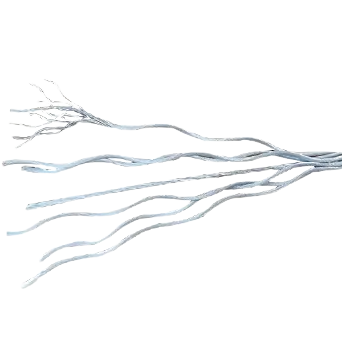
\includegraphics[scale=0.2]{rope-fiber.png}
\end{center}
    
\end{frame}

\note[itemize]{
    \item I am intentionally not going into details of fiber construction because it would be a disservice to remote attribute grammar paper
    \item Basically, its construction expresses the semantics of remote attribute grammars in classical terms
    \item Because objects implicitly carry separate values for the fields and it is like a rope that can be separated into the individual fibers
    \item But this yields an improper attribute grammar with an infinite number of attributes
    \item Then fiber approximation fixes that but it then may include cycles ...
}


\begin{frame}{Fiber Cycle Breaking}{Some fiber cycles are okay}

In RAG, some cycles can be ignored because they entirely involve so-called \alert{fiber attributes} that have no run-time significance. 

In CRAG, some cycles may carry value and will have run-time significance.
\end{frame}

\note[itemize]{
\item Even in a remote attribute grammar that is non-circular we may have fiber cycles and it's okay.
\item Fiber cycles are different between remote attribute grammar and circular remote attribute grammar because in the latter case, they may carry value. 
}



\begin{frame}{Fiber Cycle Breaking}{Issue with existing static scheduler}

Previously:
\begin{itemize}
    \item For every non-terminal whose fibered attributes take part in the cycle, created two \texttt{attribute\_decl} \alert{AST nodes} called up and down and connected all nodes to these to break cycles and preserve only UP followed by DOWN.
\end{itemize}

Now:

\begin{itemize}
    \item \alert{No creation of AST node}. Treat all nodes as either up or down. If the dependency is just fiber dependency then UP followed by DOWN. Otherwise, DOWN followed by UP.
\end{itemize}

\end{frame}

\note[itemize]{
\item Previous fiber cycle breaking module created two artificial attributes outside of the parser called UP and DOWN and this caused a lot of problems
\item To fix these we treat all attributes as either UP or DOWN and it simplified everything
}



\begin{frame}{Fiber Cycle Breaking}{Validated with RAG!}

\alert{Drop-in replacement} algorithm was successful.

\begin{itemize}
    \item Validated the algorithm against \alert{previous APS codes} that contained only fiber cycles and First and Follow APS codes
\end{itemize}

\end{frame}

\note[itemize]{
\item Tested the fiber cycle breaking algorithm against First and Follow the example.
\item And it was successful 
}



\begin{frame}{Static Scheduler}{Simplify scheduling by using groups}

Previously:
\begin{itemize}
    \item Old greedy scheduler was \alert{tightly coupled with code generation} module
\end{itemize}
    
Now:
\begin{itemize}
    \item Scheduling is still greedy but it is using groups and is simpler, easier to debug, and \alert{de-coupled from code generation} module.
    \item Includes $(\mathit{ph}, \mathit{ch})$ marker to help code generation identify the start and end of a child visit.
\end{itemize}

\end{frame}

\note[itemize]{
\item The static scheduler or the module that constructs the visit sequences was tightly coupled with the code generation module and it was not working well
\item So we designed a replacement that is still greedy but simpler as it schedules instances as groups and uses visit markers to indicate where child visit happens and when we need to return back to a parent visit from a child visit
}



\begin{frame}{Static Scheduler}{Validation in-progress ...}

\begin{itemize}
    \item Implementation is \alert{not finished yet}
\end{itemize}

\end{frame}

\note[itemize]{
\item The implementation of static schedule generation is currently in-progress but very close to being done.
}
\section{Implementation}


\begin{frame}{Static Scheduler}{Simplify scheduling by using groups}

Previously:
\begin{itemize}
    \item Old greedy scheduler was \alert{tightly coupled with code generation} module
\end{itemize}
    
Now:
\begin{itemize}
    \item Scheduling is still greedy but it is using groups and is simpler, easier to debug, and \alert{de-coupled from code generation} module
    \item Includes $(\mathit{ph}, \mathit{ch})$ marker to help code generation identify where a \alert{child visit} is happening and mark the \alert{end of parent visit}
\end{itemize}

\end{frame}


\note[itemize]{
\item Lets talk about the implementation of SCC chunk static scheduling in APS
\item The static scheduler or the module that constructs the visit sequences was tightly coupled with the code generation module and it was not working well
\item So we designed a replacement that is still greedy but simpler as it schedules instances as groups and uses visit markers to indicate where child visit happens and when parent visit ends
}




\begin{frame}{Static Schedule Assertions}{Ensuring greedy algorithm generates valid schedule}
    Due to the \alert{greedy nature of the static scheduler}, we included a series of \alert{assertions} to \alert{statically} (NOT during runtime) ensure the generated static schedule makes sense.

\newlinevspace
    
    \begin{itemize}
        \item No non-circular attribute in a circular parent visit
        \item Non-circular declared attributes may not participate in cycles
        \item Parent visits have to appear sequentially
        \item Child visits have to be invoked sequentially
        \item No missing parent and child visit
    \end{itemize}
\end{frame}

\note[itemize]{
\item Due to the greedy nature of the static scheduling algorithm we need some validation or assertions to make sure the generated schedule makes sense  
\item These validations are described in the thesis in the methods chapter
\item But some of these validations are described in this slide
}


\begin{frame}{\texttt{C} Code Statistic}{Basic Statistics About the New Scheduler}
    \begin{itemize}
        \item Old Scheduler only: $\approx500$ lines of \texttt{C} code
        \item New Static Scheduler + \alert{Assertions}: $\approx 3000$ lines of \texttt{C} code
    \end{itemize}
\end{frame}


\note[itemize]{
\item Here we have basic statistics about the new static scheduler
\item Note that the number on the second line also includes various assertion functions as well
}

\begin{frame}[fragile=singleslide]{CRAG Scala Generated Evaluator}{Attribute Instance Setter + Monotonicity check}
\begin{Verbatim}[fontsize=\scriptsize]
// Template code to support static circular evaluation
// by building upon circular evaluation structure
var changed: Boolean = false;
trait StaticCircularEvaluation[V_P, V_T] extends CircularEvaluation[V_P, V_T] {
  override def set(newValue : ValueType): Unit = {
    val prevValue = value;
    super.set(newValue);
    changed |= prevValue != value;
  }

  override def check(newValue : ValueType): Unit = {
    if (value != null) {
      if (!lattice.v_equal(value, newValue)) {
        if (!lattice.v_compare(value, newValue)) {
          throw new Evaluation.CyclicAttributeException("non-monotonic " + name);
        }
      }
    }
  }
  
  // Do not treat multiple assignments of attributes as errors
  checkForLateUpdate = false;
}
\end{Verbatim}
\end{frame}


\note[itemize]{
\item This is an example of an attribute instance setter, notice that we have a monotonicity checker that compares the old value with the new value to make sure the monotonicity requirement is being followed
\item We allow multiple attribute value assignments as this is an attribute that was declared circular 
\item We also have a global changed variable that we set if there was a \enquote{change} in attribute value after the assignment
\item In the next slide we will see how this \enquote{changed} global variable is being used
}

% kill scala codes, especially this
\begin{frame}[fragile=singleslide]{CRAG Scala Generated Evaluator}{Fixed-Point Loop around visits}
\begin{Verbatim}[fontsize=\scriptsize]
// Example of how child visits can be wrapped inside of the do-while loop
// Backup previous (global) changed value and run the code block at least once
val prevChanged_2_0 = changed;
do {
  changed = false;
  visit_4_2(v_prods);
} while (changed);
// Restore the changed value to ensure the fixed-point loop does not interfere
// with potential other fixed-point loops somewhere higher in the tree
changed = prevChanged_2_0;
\end{Verbatim}
\end{frame}

\note[itemize]{
\item Notice that \enquote{changed} global variable is being backed up before we get to the fixed-point loop and restored after the fixed-point loop
\item And then we see a do-while loop while there is a change somewhere in the attribute instances that are being re-evaluated during the visit subroutine call
}

\begin{frame}{Concession}{Concession in the implementation}
    \alert{Concession} in the implementation was \alert{no support for conditional cycles}

    \newlinevspace 
    There are two situations that can arise when using conditions with circular attribute grammars:
    
    \begin{itemize}
        \item[] \cmark \; \alert{Conditions inside the cycle}, which showcases the need to use direct edges for scheduling chunks because of potential scoping issues (\texttt{cycle-series.aps})
        \item[] \xmark \; Conditional cycles where the \alert{condition sits outside controlling the cycles}, this is where our APS implementation is not supported (\texttt{tiny-coag.aps})
    \end{itemize}
\end{frame}

\note[itemize]{
\item There are two types of the conditions with cycles, we can have a condition inside the cycle and condition outside of the cycle. The first one is supported and the second on is not
\item This is a small concession in the implementation that we left-out as a future work
\item There is a graph of an example of such attribute grammar in the thesis
\item In APS, we statically detect if a given attribute grammar has this type of a condition and we throw an error
}

\section{Conclusion}

\begin{frame}{Summary}{What has been done so far}

\begin{itemize}
    \item Defined circular remote attribute grammar
    \item Defined a valid schedule for CRAG
    \item Defined visit sequence for CRAG
    \item \alert{Proposed} an algorithm to statically evaluate CRAG
\end{itemize}
\end{frame}

\begin{frame}{Next Steps}{Coding + Testing + Benchmarking}

\begin{itemize}
    \item \alert{Implementation} of visit sequence evaluation for CRAG in APS
    \item Statically scheduling First and Follow to validate our work
    \item Statically scheduling \emph{Cool} compiler semantic analyzer
    \item Benchmarking APS implementation against JastAdd
\end{itemize}

\end{frame}





\begin{frame}{Acknowledgement}{}
    {\huge \alert{Thank you!}}
    
    \emptyline
    
    \emptyline
    
    \textbf{Advisor}: Dr. Boyland (\url{boyland@uwm.edu})
    
    \emptyline
    
    \textbf{Thesis committee members:}
        \begin{itemize}
            \item Dr. McLeod (\url{kevinm@uwm.edu})
            \item Dr. Munson (\url{munson@uwm.edu})
            \item Dr. Zhao (\url{tzhao@uwm.edu})
            \item Dr. Xu (\url{gxu4uwm@uwm.edu})
        \end{itemize}
    
\end{frame}

\begin{frame}{Reference}{}
{\tiny \fontsize{1.5}{4}\selectfont
\bibliographystyle{alpha}
\bibliography{references}{}
}
\end{frame}



\end{document}


